\documentclass[12pt,a4paper]{article}
\usepackage[utf8]{inputenc}
\usepackage[T2A]{fontenc}
\usepackage[russian]{babel}
\usepackage[left=2.5cm,right=2cm,top=2cm,bottom=2cm]{geometry}
\usepackage{graphicx}
\usepackage{amsmath,amssymb}
\usepackage{booktabs}
\usepackage{tabularx}
\usepackage{listings}
\usepackage{xcolor}
\usepackage{tocloft}
\usepackage[hidelinks]{hyperref}

% Настройка оглавления: отточия и аккуратные отступы
\renewcommand{\cftsecleader}{\cftdotfill{\cftdotsep}}
\setlength{\cftbeforesecskip}{5pt}
\setlength{\cftbeforesubsecskip}{2pt}

\definecolor{codegreen}{rgb}{0,0.6,0}
\definecolor{codegray}{rgb}{0.5,0.5,0.5}
\definecolor{codepurple}{rgb}{0.58,0,0.82}
\definecolor{backcolour}{rgb}{0.96,0.96,0.96}

\lstdefinestyle{mystyle}{
    backgroundcolor=\color{backcolour},
    commentstyle=\color{codegreen},
    keywordstyle=\color{blue}\bfseries,
    numberstyle=\tiny\color{codegray},
    stringstyle=\color{codepurple},
    basicstyle=\ttfamily\scriptsize,
    breakatwhitespace=false,
    breaklines=true,
    captionpos=b,
    keepspaces=true,
    numbers=left,
    numbersep=5pt,
    showspaces=false,
    showstringspaces=false,
    showtabs=false,
    tabsize=2
}
\lstset{style=mystyle}

\begin{document}

% --- ТИТУЛЬНЫЙ ЛИСТ СТРОГО ПО ШАБЛОНУ ---
\begin{titlepage}
    \centering
    {\bfseries\large МОСКОВСКИЙ АВИАЦИОННЫЙ ИНСТИТУТ\par
    (НАЦИОНАЛЬНЫЙ ИССЛЕДОВАТЕЛЬСКИЙ УНИВЕРСИТЕТ)\par}
    \vspace{0.8cm}
    Институт №8 «Компьютерные науки»\par
    \vspace{3.5cm}
    {\bfseries\Large Лабораторная работа №1\par}
    \vspace{0.3cm}
    {\large по курсу «Программирование графических процессоров»\par}
    \vspace{0.8cm}
    {\bfseries\large Освоение программного обеспечения для работы с технологией CUDA.\par Примитивные операции над векторами\par}
    \vspace{4cm}
    \begin{flushleft}
    \hspace*{7.5cm}
    \begin{minipage}{8cm}
        Выполнил: Л.А. Фокин\\[0.3cm]
        Группа: М8О-401Б-23\\[0.3cm]
        Преподаватель:  А.Ю. Морозов
    \end{minipage}
    \end{flushleft}
    \vfill
    {\large Москва, 2026}
\end{titlepage}

\tableofcontents
\newpage

\section{Условие}
\subsection*{Цель работы и общая постановка задачи}
Целью лабораторной работы является ознакомление и освоение программного обеспечения для разработки параллельных приложений на архитектуре NVIDIA CUDA, а также практическая реализация базовой векторной операции с использованием ресурсов графического ускорителя и оценка достигнутого ускорения.

\subsection*{Вариант задания}
\textbf{Вариант 1. Сложение векторов.}
\begin{itemize}
    \item \textbf{Входные данные:} На первой строке задано целое число $n$ — размер векторов ($n < 2^{25}$). В следующих двух строках записано по $n$ вещественных чисел типа \texttt{double} — элементы первого и второго векторов соответственно.
    \item \textbf{Выходные данные:} Вывести $n$ чисел — результат поэлементного сложения исходных векторов. Все результаты выводятся с относительной точностью $10^{-10}$ в экспоненциальной форме.
\end{itemize}

\section{Программное и аппаратное обеспечение}
\subsection*{Аппаратное обеспечение}
\begin{itemize}
    \item \textbf{Графический процессор (GPU):} NVIDIA GeForce RTX 5070
    \begin{itemize}
        \item Compute Capability: 12.0
        \item Объем глобальной памяти (Global Memory): 12\,792 МБ ($\approx 12$ ГБ) GDDR7
        \item Объем разделяемой памяти на блок (Shared Memory): 49\,152 байт (48 КБ)
        \item Объем константной памяти (Constant Memory): 65\,536 байт (64 КБ)
        \item Количество 32-битных регистров на блок: 65\,536
        \item Максимальное количество нитей на блок: 1024
        \item Максимальный размер блока: $(1024, 1024, 64)$
        \item Максимальный размер сетки: $(2147483647, 65535, 65535)$
        \item Количество потоковых мультипроцессоров (SM): 48
    \end{itemize}
    \item \textbf{Центральный процессор (CPU):} AMD Ryzen 5 8400F 6-Core Processor (6 физических ядер, 12 логических потоков, базовая тактовая частота 4.2 ГГц, Max Boost до 4.7 ГГц, кэш L3 16 МБ)
    \item \textbf{Оперативная память (RAM):} 16 ГБ DDR5
    \item \textbf{Жесткий диск (Накопитель):} NVMe Solid State Drive (SSD) емкостью 1 ТБ (раздел \texttt{/dev/sdd}, файловая система ext4)
\end{itemize}

\subsection*{Программное обеспечение}
\begin{itemize}
    \item \textbf{Операционная система (OS):} Ubuntu 24.04 LTS (x86\_64 Linux kernel 6.6.87)
    \item \textbf{Среда разработки (IDE / Редактор):} Zed Editor / Visual Studio Code
    \item \textbf{Компилятор CUDA:} NVIDIA CUDA Compiler Driver (nvcc) v12.0 (V12.0.140)
    \item \textbf{Компилятор C++ хоста:} g++ (Ubuntu 13.3.0)
\end{itemize}

\section{Метод решения}
Операция поэлементного сложения векторов $\vec{C} = \vec{A} + \vec{B}$ выражается формулой $C[i] = A[i] + B[i]$ для всех $i \in [0, n - 1]$. Операция не содержит информационных зависимостей между элементами (Data Dependency), что позволяет параллельно вычислять каждый элемент в отдельном аппаратном потоке GPU.

Для обработки произвольного объема данных при фиксированной сетке потоков применяется идиома \textbf{Grid-Stride Loop}:
\begin{lstlisting}[language=C++]
int idx = blockIdx.x * blockDim.x + threadIdx.x;
int offset = blockDim.x * gridDim.x;
for (int i = idx; i < n; i += offset) {
    a[i] += b[i];
}
\end{lstlisting}
Потоки стартуют со своего глобального индекса \texttt{idx} и сдвигаются с шагом \texttt{offset}, равным общему числу потоков в запущенной сетке ($\text{gridDim.x} \times \text{blockDim.x}$). Это позволяет:
\begin{enumerate}
    \item Зафиксировать аппаратную конфигурацию блоков и нитей, исключив зависимость числа создаваемых потоков от размера входного вектора $n$;
    \item Обеспечить объединение обращений к глобальной памяти (Coalesced Memory Access): последовательные потоки одного варпа одновременно читают непрерывные 64-битные сегменты \texttt{double}, минимизируя число транзакций контроллера памяти.
\end{enumerate}

\subsection*{Использованные источники}
\begin{enumerate}
    \item NVIDIA Corporation. \textit{CUDA C++ Programming Guide (Release 12.x)}. URL: \url{https://docs.nvidia.com/cuda/cuda-c-programming-guide/}.
    \item Воеводин В. В., Воеводин Вл. В. \textit{Параллельные вычисления}. — СПб.: БХВ-Петербург, 2002.
    \item Морозов А. Ю. \textit{Курс лекций по программированию графических процессоров (CUDA)}. МАИ, 2024.
\end{enumerate}

\newpage
\section{Описание программы}
Программа декомпозирована на исходный модуль на языке CUDA C++ (\texttt{main.cu}) и сборочный конфигурационный файл (\texttt{Makefile}).

\subsection*{Основные типы данных и функции}
\begin{itemize}
    \item \textbf{Типы данных:}
    \begin{itemize}
        \item \texttt{double} — вещественные числа повышенной точности (64 бит, стандарт IEEE 754) для элементов векторов;
        \item \texttt{int} — целочисленные счетчики индексов, размер вектора $n$ и параметры конфигурации сетки (число блоков и нитей);
        \item \texttt{cudaError\_t} — тип кода возврата функций CUDA API.
    \end{itemize}
    \item \textbf{Макрос \texttt{CSC}:} перехватывает ошибки функций CUDA API, печатает сообщение в поток \texttt{stderr} с указанием файла, строки и описания через \texttt{cudaGet\-Error\-String}, после чего безопасно завершает работу программы с кодом \texttt{0}.
    \item \textbf{Ядро \texttt{vector\_add}:} функция \texttt{\_\_global\_\_}, выполняющая сложение элементов double по схеме grid-stride.
    \item \textbf{Функция \texttt{main}:} выполняет быстрый потоковый ввод, выделяет память на хосте (\texttt{malloc}) и устройстве (\texttt{cudaMalloc}), копирует данные на GPU (\texttt{cudaMemcpyHost\-ToDevice}), запускает ядро, синхронизирует GPU (\texttt{cudaDeviceSynchronize}), считывает результат обратно и выводит значения в формате \texttt{std::scientific} с точностью $10^{-10}$ с заменой $-0.0$ на $0.0$.
\end{itemize}

\subsection*{Исходный код программы (\texttt{main.cu})}
\lstinputlisting[language=C++]{main.cu}

\newpage
\section{Результаты}
В соответствии с требованиями были выполнены сравнительные замеры производительности на CPU и GPU на различных масштабах данных ($N = 100\,000$, $N = 5\,000\,000$ и предельный тест $N = 20\,000\,000$) для различных конфигураций сетки (от $\ll 1, 32 \gg$ до $\ll 1024, 1024 \gg$). Единицы измерения времени — миллисекунды (мс).

\begin{table}[htbp]
\centering
\small
\setlength{\tabcolsep}{4.5pt}
\caption{Сравнение времени работы (мс) и ускорения на CPU и GPU}
\vspace{0.2cm}
\begin{tabular*}{\textwidth}{@{\extracolsep{\fill}} r c r r r r r @{}}
\toprule
\textbf{Размер} & \textbf{Сетка} & \textbf{CPU} & \textbf{GPU Ядро} & \textbf{GPU Всего} & \textbf{Ускорение} & \textbf{Полное} \\
$\mathbf{N}$ & $\mathbf{\ll B, T \gg}$ & \textbf{(мс)} & \textbf{(мс)} & \textbf{(мс)} & \textbf{ядра} & \textbf{ускорение} \\
\midrule
100\,000 & $\ll 1, 32 \gg$ & 0.033 & 0.585 & 1.133 & 0.06x & 0.03x \\
100\,000 & $\ll 1, 256 \gg$ & 0.033 & 0.197 & 0.792 & 0.17x & 0.04x \\
100\,000 & $\ll 1, 1024 \gg$ & 0.033 & 0.121 & 0.633 & 0.27x & 0.05x \\
100\,000 & $\ll 32, 256 \gg$ & 0.033 & 0.066 & 0.628 & 0.50x & 0.05x \\
100\,000 & $\ll 256, 256 \gg$ & 0.033 & 0.063 & 0.601 & 0.53x & 0.06x \\
100\,000 & $\ll 1024, 256 \gg$ & 0.033 & 0.259 & 0.980 & 0.13x & 0.03x \\
100\,000 & $\ll 1024, 1024 \gg$ & 0.033 & 0.129 & 0.631 & 0.26x & 0.05x \\
5\,000\,000 & $\ll 1, 32 \gg$ & 2.181 & 84.169 & 101.912 & 0.03x & 0.02x \\
5\,000\,000 & $\ll 1, 256 \gg$ & 2.181 & 9.993 & 26.903 & 0.22x & 0.08x \\
5\,000\,000 & $\ll 1, 1024 \gg$ & 2.181 & 3.413 & 19.039 & 0.64x & 0.12x \\
5\,000\,000 & $\ll 32, 256 \gg$ & 2.181 & 0.416 & 16.176 & 5.25x & 0.14x \\
5\,000\,000 & $\ll 256, 256 \gg$ & 2.181 & 0.418 & 17.434 & 5.22x & 0.12x \\
5\,000\,000 & $\ll 1024, 256 \gg$ & 2.181 & 0.307 & 16.846 & 7.11x & 0.13x \\
5\,000\,000 & $\ll 1024, 1024 \gg$ & 2.181 & 0.324 & 17.893 & 6.74x & 0.12x \\
20\,000\,000 & $\ll 1, 32 \gg$ & 10.403 & 295.995 & 358.010 & 0.04x & 0.03x \\
20\,000\,000 & $\ll 1, 256 \gg$ & 10.403 & 35.359 & 94.572 & 0.29x & 0.11x \\
20\,000\,000 & $\ll 1, 1024 \gg$ & 10.403 & 9.873 & 71.125 & 1.05x & 0.15x \\
20\,000\,000 & $\ll 32, 256 \gg$ & 10.403 & 2.138 & 58.716 & 4.87x & 0.18x \\
20\,000\,000 & $\ll 256, 256 \gg$ & 10.403 & 0.944 & 58.143 & 11.02x & 0.18x \\
20\,000\,000 & $\ll 1024, 256 \gg$ & 10.403 & 1.428 & 60.951 & 7.28x & 0.17x \\
20\,000\,000 & $\ll 1024, 1024 \gg$ & 10.403 & 0.928 & 60.759 & 11.21x & 0.17x \\
\bottomrule
\end{tabular*}
\end{table}

\begin{figure}[htbp]
    \centering
    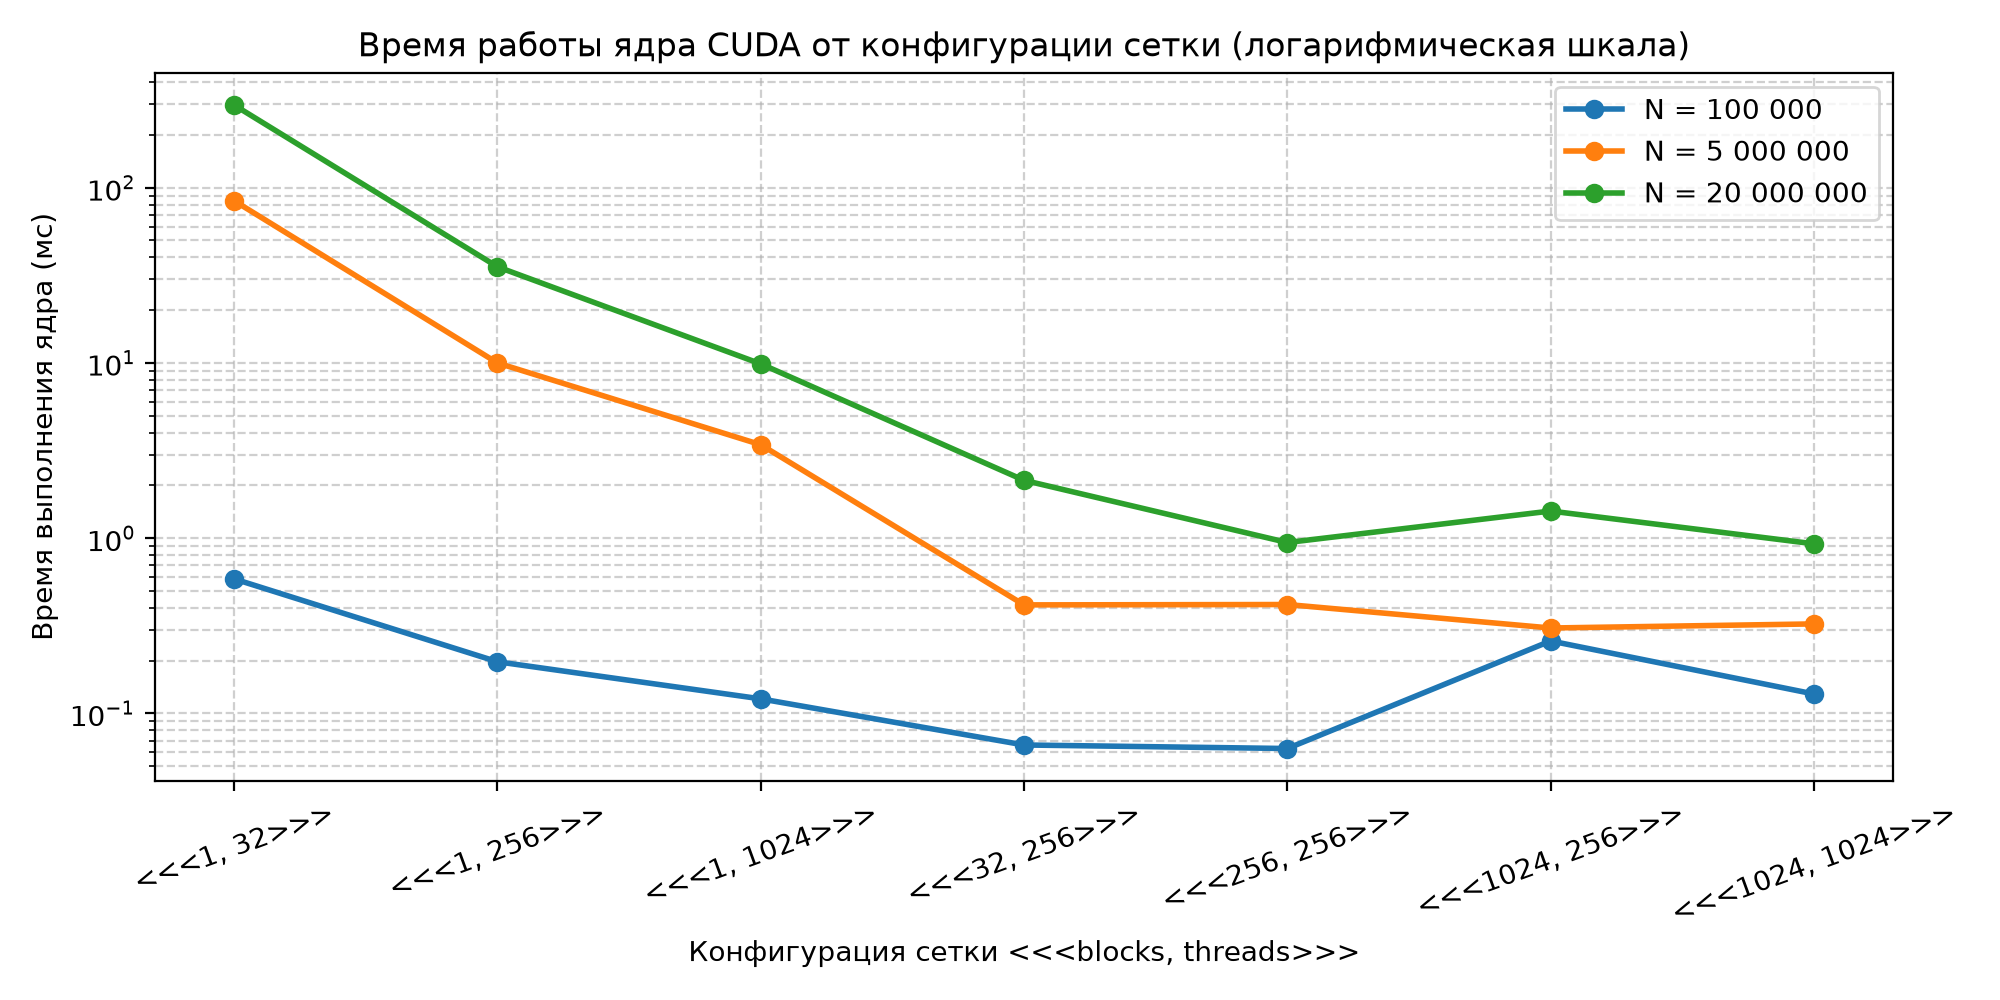
\includegraphics[width=0.88\textwidth]{plot_configs.png}
    \caption{Зависимость времени выполнения ядра от конфигурации сетки (лог. шкала)}
\end{figure}

\begin{figure}[htbp]
    \centering
    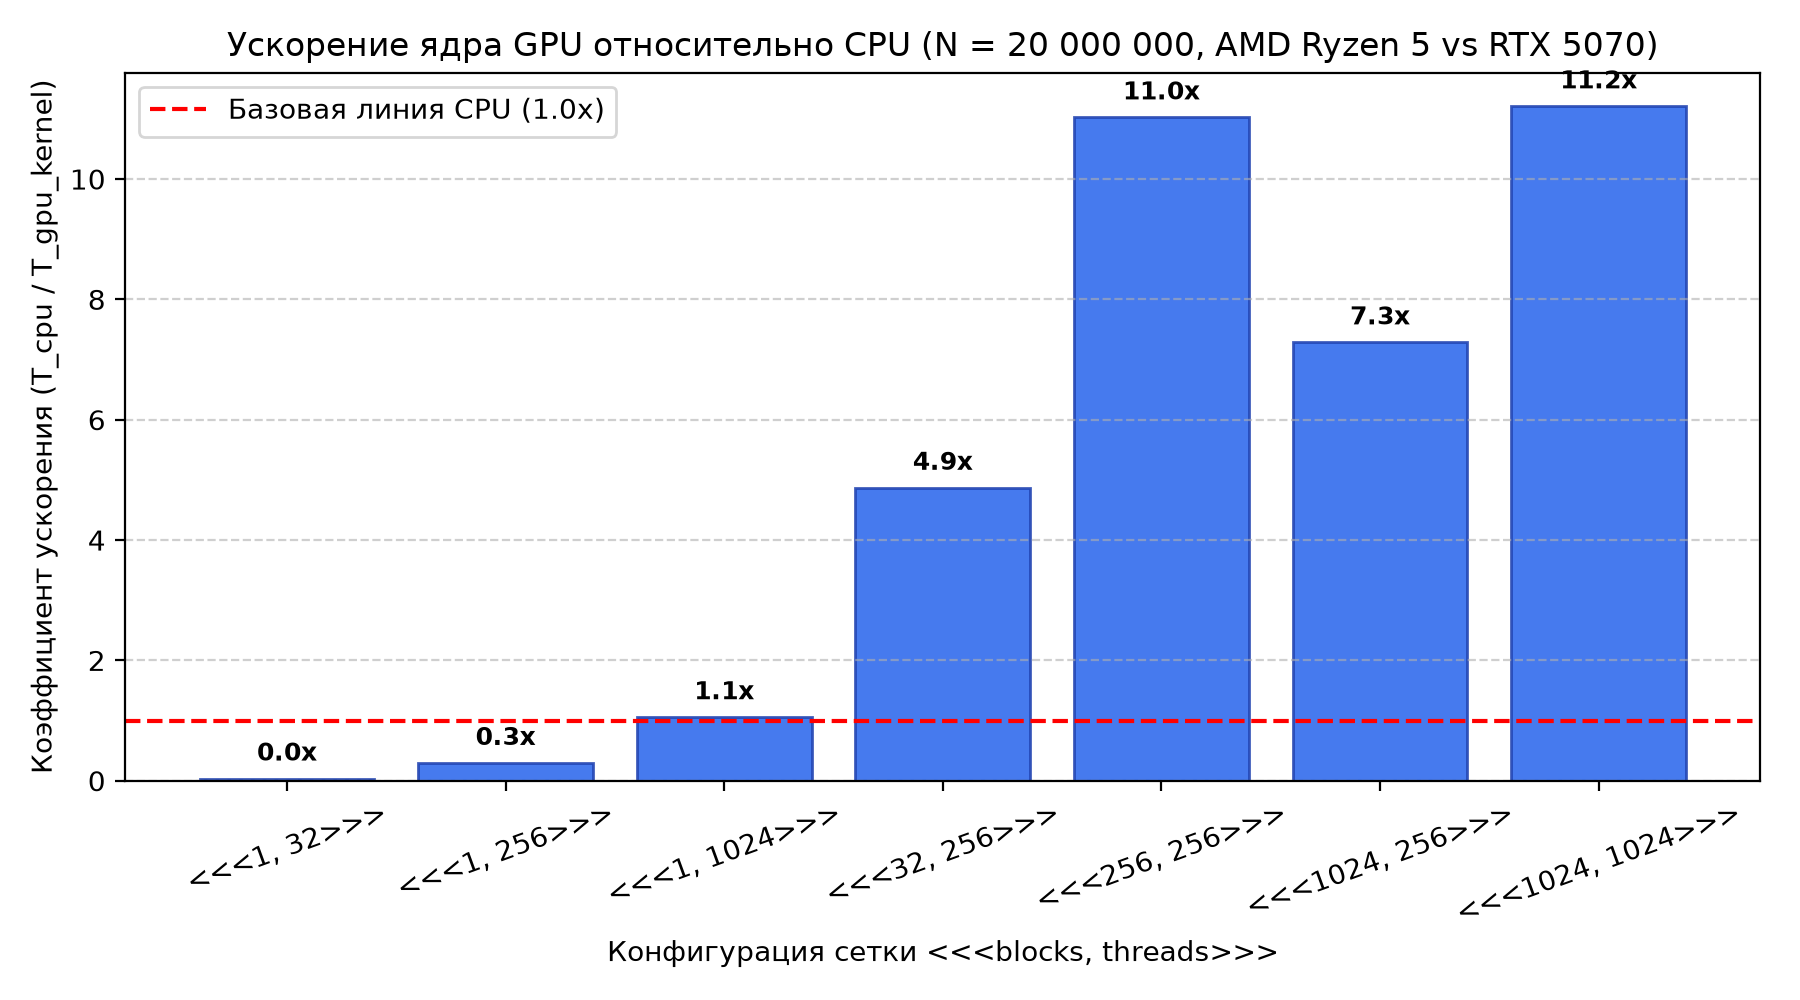
\includegraphics[width=0.85\textwidth]{plot_speedup.png}
    \caption{Ускорение вычислительного ядра GPU относительно CPU ($N = 20\,000\,000$)}
\end{figure}

\newpage
\section{Выводы}
\subsection*{Область применения алгоритма и типовые задачи}
Операция векторного сложения является фундаментальным примитивом линейной алгебры (уровень BLAS-1, операция \texttt{AXPY}).
Типовые прикладные задачи, использующие данный алгоритм:
\begin{itemize}
    \item Машинное обучение: пошаговое обновление весов моделей (Stochastic Gradient Descent / Adam) в нейронных сетях;
    \item Физическое математическое моделирование: решение систем дифференциальных уравнений методом Эйлера и Рунге-Кутты (накопление приращений физических величин);
    \item Цифровая обработка сигналов: наложение сигналов и спектральное сложение.
\end{itemize}

\subsection*{Оценка сложности программирования и возникшие проблемы}
\begin{itemize}
    \item \textbf{Сложность программирования:} Алгоритмическая сложность по времени составляет $O(N)$, по дополнительной памяти на GPU — $O(1)$ поверх входных массивов. Реализация прямолинейна ввиду полного отсутствия зависимости по данным между соседними итерациями.
    \item \textbf{Возникшие проблемы:}
    \begin{enumerate}
        \item На малых размерностях входных векторов ($N = 100\,000$) накладные расходы на копирование данных через шину PCI-Express существенно превосходят время чистых вычислений;
        \item При форматировании вывода в стандартном потоке C++ \texttt{std::scientific} нулевые значения с плавающей точкой после сложения с отрицательными числами могли принимать значение $-0.0000000000\text{e}+00$, что потребовало явной нормализации перед печатью.
    \end{enumerate}
\end{itemize}

\subsection*{Сравнение и объяснение полученных результатов}
Эксперименты наглядно подтвердили архитектурные особенности параллелизма SIMT:
\begin{enumerate}
    \item При конфигурации с одним варпом ($\ll 1, 32 \gg$) время работы ядра на $N = 20\,000\,000$ составляет $295.99$ мс, в то время как при полной загрузке мультипроцессоров ($\ll 256, 256 \gg$) время сокращается до $0.94$ мс (ускорение в $315$ раз).
    \item На предельных массивах ($N = 20\,000\,000$) ядро GPU RTX 5070 обгоняет процессор AMD Ryzen 5 более чем в $11$ раз ($0.93$ мс против $10.40$ мс), наглядно подтверждая преимущество пропускной способности видеопамяти GDDR7.
\end{enumerate}

\end{document}
